% Constructed and checked from the problem; not a geometric proof.
\documentclass[tikz,border=8pt]{standalone}
\begin{document}
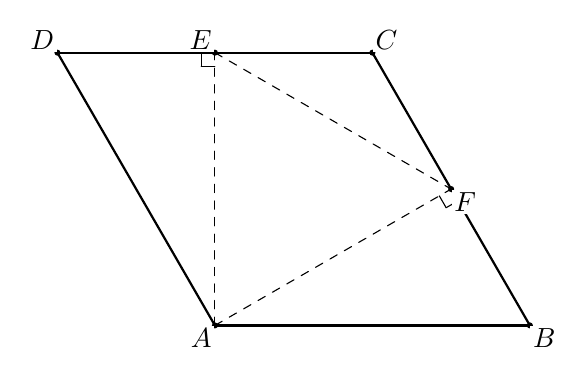
\begin{tikzpicture}[scale=1,line cap=round,line join=round]
\coordinate (p0) at (0,0);
\coordinate (p1) at (4,0);
\coordinate (p2) at (2,3.4641016);
\coordinate (p3) at (-2,3.4641016);
\coordinate (p4) at (0,3.4641016);
\coordinate (p5) at (3,1.7320508);
\draw[thick] (p0) -- (p1);
\draw[thick] (p1) -- (p2);
\draw[thick] (p3) -- (p2);
\draw[thick] (p3) -- (p0);
\draw[dashed] (p0) -- (p4);
\draw[dashed] (p0) -- (p5);
\draw[dashed] (p4) -- (p5);
\draw (0,3.2907016) -- (-0.1734,3.2907016);
\draw (-0.1734,3.2907016) -- (-0.1734,3.4641016);
\draw (2.8498312,1.6453508) -- (2.9365312,1.495182);
\draw (2.9365312,1.495182) -- (3.0867,1.581882);
\fill (p0) circle (1.1pt) node[fill=white,inner sep=1pt,below left] {$A$};
\fill (p1) circle (1.1pt) node[fill=white,inner sep=1pt,below right] {$B$};
\fill (p2) circle (1.1pt) node[fill=white,inner sep=1pt,above right] {$C$};
\fill (p3) circle (1.1pt) node[fill=white,inner sep=1pt,above left] {$D$};
\fill (p4) circle (1.1pt) node[fill=white,inner sep=1pt,above left] {$E$};
\fill (p5) circle (1.1pt) node[fill=white,inner sep=1pt,below right] {$F$};
\end{tikzpicture}
\end{document}
